
\documentclass[11pt, hide notes]{beamer} % Font sizes: 8, 9, 10, 11, 12, 14, 17, 20. Some sizes require "extsizes" package to be installed.
%%%%%%%%%%%%%%%%%%%%%%%%%%%%%%%%%%%%%%%%%%%%%%%%%%%%%%%%%%%%%%%%%%%%%%%%%%%%%%%%%%%%%%
%\usepackage{beamerthemeshadow}
\usepackage{graphics}
\usepackage{graphicx} % Enable the use of graphs
\usepackage{amsfonts} % Enable special mathemtical characters.
\usepackage{amsmath}  % Enable the use  Multi-line equations, compound symbols, etc
\usepackage{extsizes} % Enable the use of different font sizes.
\usepackage{booktabs} % More complex tables
\usepackage{hyperref} % Links
\usepackage{scalefnt} % Redução do tamanho das tabelas
\usepackage{subfig}   % Subfigures
\usepackage{helvet}   % Different fonts
\usepackage{arydshln}
\usepackage{pdfpages}
\usepackage{beamerthemesplit}
\usefonttheme[onlymath]{serif}

% Need also to download pgf, ms and xcolor packages.
\usepackage[ansinew]{inputenc} % Permite digitar os acentos diretamente.
\usepackage[portuguese]{babel} % Habilita a língua portuguesa

\usetheme{Copenhagen} % Options: default, Antibes, Berkeley, Berlin, Copenhagen, Madrid, Pittsburgh, Singapore, Boadilla, etc.

\useinnertheme{circles} % Options: default, circles, rectangles, rounded, inmargin,
%\useoutertheme{default} % Options: default, infolines, miniframes, etc. Options []: footline=empty, footline=authorinstitute, footline=authortitle, footline=institutetitle, footline=authorinstitutetitle, subsection=.true or false.

%\usecolortheme{beetle} % Options: default, beetle, albatross, crane, fly, wolverine, beaver, whale, etc.
%\useinnertheme{orchid} % Inner Color Themes: lily, orchid, rose
%\useoutertheme{dolphin} % Outer Color Themes: whale, seahorse, dolphin

\setbeamersize{text margin left=0.6cm, text margin right=0.6cm}

\setbeameroption{hide notes} % Use this option instead in presentations with projectors: show notes on second screen
% to add notes, type: \note[item]<1>{Text}

\begin{document}

\title[Aula 01]{Beamer - Aula 01}
%\subtitle{Preliminar e Incompleto. Coment�rios e sugest�es s�o bem-vindos!}


\author[Besarria(2022)]{Cássio da Nóbrega Besarria }


\date[]{João Pessoa, 22 de agosto de 2017}

\setbeamercovered{dynamic}


\beamertemplatenavigationsymbolsempty


\begin{frame}
\titlepage
\end{frame}



\begin{frame}
	\frametitle{Resumo}
	%\tableofcontents[pausesections] % Use option part=* to specify each part if you want to include a reminder of the outline before each section.
	\tableofcontents
\end{frame}



\section{Economia e Finanças Públicas}


\begin{frame}[label=myslide01] % [<options>=label, plain, (c=center,t=top,b=bottom)]

\frametitle{Economia e Finanças Públicas} {\ % <= Be careful with this!

    \begin{itemize}
\pause \item Quem deve deve suportar o esforço da redução déficit fiscal:
\pause \item Funcionários públicos, cidadãos em geral ou empresas?
    \end{itemize}
     
    }  % <= Be careful with this!
\end{frame}


\section{Governo democrático, estado e sociedade}
\frame{\sectionpage}


\frame
{
  \frametitle{O que é um governo democrático?}

\begin{itemize}	
	\pause \item As democracias liberais dos países mais desenvolvidos assentam numa separação entre o poder executivo (governo), legislativo (assembleia legislativa) e o poder judiciário (tribunais). 
	\pause \item Um governo democrático é uma instituição dotada de poderes delimitados por lei, composto por uma equipe de pessoas com um líder cuja legitimidade advém do processo de competição política pelo voto popular.
\end{itemize}
 
}

\begin{frame}[label=myslide14] % [<options>=label, plain, (c=center,t=top,b=bottom)]
	
	\frametitle{Avaliação das Políticas Públicas} {\ % <= Be careful with this!
		

\begin{itemize}	
	\pause \item Para avaliar ou comparar pol�ticas alternativas � preciso estabelecer um crit�rio. 
	\pause \item Objetivo �nico? Utilidade.
	\pause \item Qual Utilidade? Inst�ntanea (consumo, lazer),
	Intertemporal (investimento, taxa de desconto).
	\pause \item Utilidade Agregada? Utilitarista, Rawlsiana,...
\end{itemize}

}
\end{frame}

\begin{frame}[label=myslide4.1] % [<options>=label, plain, (c=center,t=top,b=bottom)]
	
	\frametitle{Restri��o or�ament�ria do governo} {\ % <= Be careful with this!
		
		\begin{figure}
			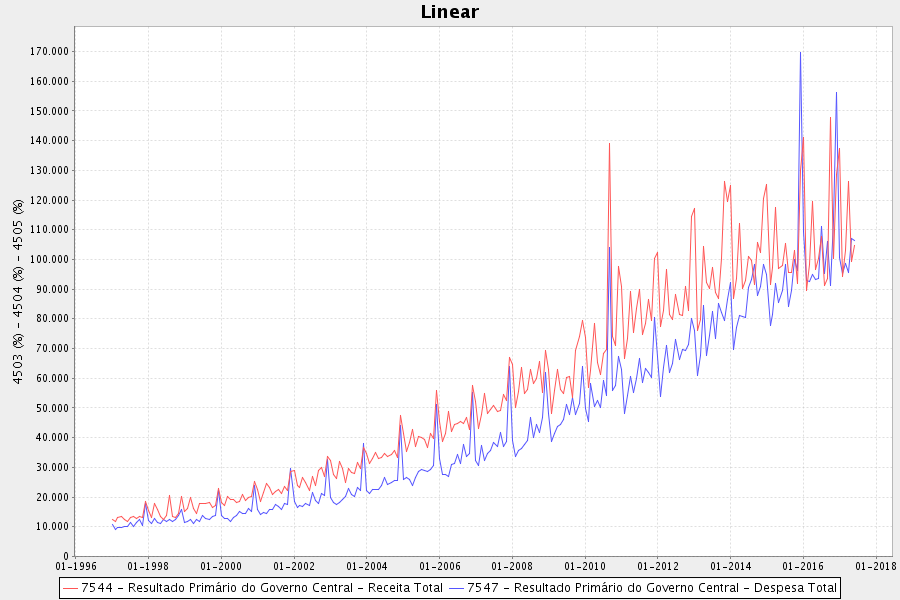
\includegraphics[scale=0.3]{fig1.png}
			\label{fig1} 
			\caption{Receita e despesa total} 
		\end{figure}
		
	}  % <= Be careful with this!
\end{frame}

\begin{frame}[label=myslide06] % [<options>=label, plain, (c=center,t=top,b=bottom)]
	
	\frametitle{Impostos atuais versus impostos futuros} {\ % <= Be careful with this!
		
A d�vida no per�odo 2 ser�:
		
\begin{equation}
B_2=(1+r)B_1+(G_2-T_2)
\label{obj4}
\end{equation}
assumindo $B_2=0$ e $B_1=1$, temos:

\begin{equation}
\frac{B_t}{Y_t}-\frac{B_{t-1}}{Y_{t-1}}=(r-g)\left(\frac{B_{t-1}}{Y_{t-1}}\right)+\frac{G_t-T_t}{Y_t}
\label{obj10}
\end{equation}		
				
	}  % <= Be careful with this!
\end{frame}

\begin{frame}[label=myslide14] % [<options>=label, plain, (c=center,t=top,b=bottom)]
	
	\frametitle{Equidade} {\ % <= Be careful with this!
		
		Distribui��o do �nus tribut�rio deve ser equitativa entre os indiv�duos da sociedade (cada indiv�duo deve contribuir com uma parcela 'justa' para cobrir os custos do governo). \\ \vspace{1cm}
		
		\textbf{Princ�pio}: Cada indiv�duo deveria contribuir
		com uma quantidade proporcional aos benef�cios gerados
		pelo consumo do bem p�blico (dificuldade: estabelecer uma
		regra geral � indiv�duos n�o declaram o valor dado ao
		benefício); 
		
	}
\end{frame}

\begin{frame}[label=myslide16.5] % [<options>=label, plain, (c=center,t=top,b=bottom)]
	
	\frametitle{Impostos indiretos ou sobre consumo} {\ % <= Be careful with this!
		
		% Table generated by Excel2LaTeX from sheet 'Plan1'
		
		\begin{table}[H]
			\centering
			\caption{Exemplo da cesta básica}
			\vspace{-0.40cm}
			\begin{tabular}{@{}l|p{1cm}p{1cm}ccp{1.7cm}}
				\midrule
				& Renda (R\$) & Cons. (R\$) & Cons./Renda & Trib. (10\%) & Trib./Renda \\
				\midrule
				Indiv. 01 & 1.000 & 800   & 80    & 80    & 8 \\
				Indiv. 02 & 10.000 & 5.500 & 55    & 550   & 5.5 \\
				\bottomrule
			\end{tabular}%
			\label{tab1}%
		\end{table}%
		
	}
\end{frame}

\begin{frame}[label=myslide16.6] % [<options>=label, plain, (c=center,t=top,b=bottom)]
	
	\frametitle{Cálculo do imposto por dentro e por fora} {\ % <= Be careful with this!
		
		\begin{table}[H]
			\centering
			\caption{Imposto por dentro (ICMS)}
			\begin{tabular}{l|c}
				\toprule \midrule
				Preço venda - base de cálculo (em R\$) & 257.40 \\ 
				& - \\
				Tributo (17\%) & 43.75 \\ \midrule
				Preço sem imposto & 213.65 \\
				& - \\
				Custo unitário (em R\$) & 200.00 \\ \midrule
				Lucro obtido (em R\$) & 13.65 \\
				\bottomrule
			\end{tabular}%
			\label{tab3}%
		\end{table}%
		
		
	}
\end{frame}





\end{document}
